% Author: Pakkapon Phongthawee

% !TEX program = xelatex

\documentclass[xcolor=dvipsnames, xetex,serif]{beamer}
%\documentclass[handout,xetex,serif]{beamer} %ใช้บรรทัดนี้สำหรับปริ้นเอกสาร
\usepackage{color,amsmath,graphics,graphicx}
\usepackage{epsfig,amsfonts,graphics}
\usepackage{mathrsfs,hyperref}
\usepackage{subcaption,float,framed,algorithm2e,hyperref}
%===============================================
\usepackage{fontspec,xltxtra,xunicode}
\defaultfontfeatures{Scale=1.23}
\XeTeXlinebreaklocale “th_TH” % สำหรับตัดคำ
\setmainfont[Scale=1.23]{THSarabunNew}
% 1.23 เท่าคือจาก 12 pt บน LaTeX ให้เท่ากับ 16pt บน Word
%=====================================================
%\usepackage{pgfpages} %ใช้บรรทัดนี้สำหรับปริ้นเอกสาร
%\pgfpagesuselayout{4 on 1}[a4paper,border shrink=5mm,landscape]
%\pgfpagesuselayout{2 on 1}[a4paper,border shrink=5mm]
%ใช้บรรทัดนี้สำหรับปริ้นเอกสาร

%%%%%%%%%%%%%%% THEOREM Environments %%%%%%%%%% 					
\newtheorem{conjecture}[theorem]{บทคาดการณ์}								
\newtheorem{remark}[theorem]{หมายเหตุ}										
\numberwithin{equation}{section}							
\renewcommand\tablename{ตารางที่}
\renewcommand\figurename{รูปที่}						
\renewcommand{\bibname}{บรรณานุกรม}						
\renewcommand{\indexname}{ดรรชนี}
\setbeamertemplate{caption}[numbered]	
\setbeamertemplate{theorems}[numbered]				
%%%%%%%%%%%%%%%%%%%%%%%%%%%%%%%%%%%%%%%%%%%%%%%

\mode<presentation>{
	\usetheme{Madrid}
    \usecolortheme[named=PineGreen]{structure}
}
\title[วิธีเชิงตัวเลขสำหรับต่อเติมภาพ]{\normalsize{ขั้นตอนวิธีเชิงตัวเลขชนิดใหม่สำหรับการต่อเติมภาพที่ใช้การแปรผันรวมกับการประยุกต์สำหรับซ่อมแซมภาพจิตรกรรมไทยโบราณและการลบบทบรรยายจากอนิเมะ\\A new numerical algorithm for TV-based image inpainting with its applications for restoring ancient Thai painting images and removing subtitles from animes}}
\author[ภัคพล]{ภัคพล พงษ์ทวี}
\institute[SU]{
 	ภาควิชาคณิตศาสตร์\\
 	มหาวิทยาลัยศิลปากร \\}
\date[Project Proposal]{งานประชุมวิชาการสำหรับนักศึกษาระดับปริญญาตรี\\ สาขาวิชาคณิตศาสตร์ประยุกต์ ครั้งที่ 8\\27 เมษายน 2562}
 
 \AtBeginSubsection[]{
 	\begin{frame}<beamer>
 		\frametitle{Outlines}
 		\tableofcontents [currentsection,currentsubsection]
     \end{frame}
}
%\setbeamertemplate{item}[square]
%============================================================================
\begin{document}
    \begin{frame}
        \titlepage 
    \end{frame}
    \begin{frame}
        \frametitle{การต่อเติมภาพ (Image Inpainting)} 
        \begin{figure}[H]
            \centering
            \begin{subfigure}{0.3\linewidth}
                \centering
                
\includegraphics[width=0.8\linewidth]{images/grayscale_inpaint/toinpaint.png}
                \caption{ภาพที่ต้องการซ่อมแซม}
                %note{การต่อเติมภาพ เป็นวิธีการประมวลผลภาพชนิดหนึ่งมีเป้าหมายเพื่อซ่อมแซมภาพด้วยการต่อเติมข้อมูลของความเข้มของสีบนบริเวณที่กำหนด (ต่อไปจะเรียกบริเวณนี้ว่าโดเมนต่อเติม) โดยอาศัยข้อมูลของความเข้มของสีที่ปรากฏในภาพ จากภาพต้องการต่อเติมพื้นที่สีขาว ซึ่งเมื่อต่อเติมแล้วจะได้ภาพดังนี้}
            \end{subfigure}
            \begin{subfigure}{0.3\linewidth}
                \centering
                
\includegraphics[width=0.8\linewidth]{images/grayscale_inpaint/inpaintdomain.png}
                \caption{โดเมนต่อเติม}
            \end{subfigure}
            \begin{subfigure}{0.3\linewidth}
                \centering
                
\includegraphics[width=0.8\linewidth]{images/grayscale_inpaint/result_splitbergman.png}
                \caption{ภาพที่ได้รับการซ่อมแซม}
            \end{subfigure}
            \caption{ตัวอย่างการซ่อมแซมภาพ}
            \label{fig1}
        \end{figure}
    \end{frame}
    \begin{frame}
        \frametitle{ปัญหาการต่อเติมภาพ}
        \begin{itemize}
            \item[(1)] การต่อเติมภาพเฉดเทา
            \item[(2)] การต่อเติมภาพสี
        \end{itemize}
    \end{frame}
    \begin{frame}
        \frametitle{ภาพเฉดเทา}
        \begin{itemize}
            \item โดเมนภาพ (image domain) $\Omega \subset \mathbb{R}^2$ 
            \item โดเมนต่อเติม (inpainting domain)  $ D \subset \mathbb{R}^2$
            \item พิกัดทางกายภาพ (physical position) $ \mathbf{x} = (x,y) \in \Omega $ 
            \item ระดับความเข้มของภาพ (image intensity)  $V \subset [0,\infty)$ 
            \item ภาพเฉดเทา (grayscale image) $ u: \Omega \rightarrow V,\ z: \Omega \rightarrow V$
            \item โดยไม่เสียหลักการสำคัญ $ \Omega = [1,n]^2 $ และ $ V = [0,1] $ เมื่อ $n>0$ เป็นจำนวนเต็มบวก 
        \end{itemize}
         \begin{figure}[h]
            \[
            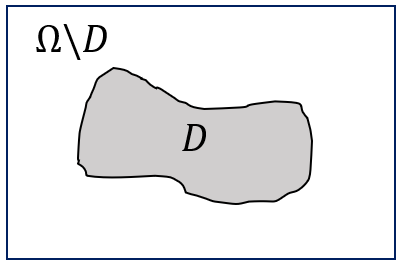
\includegraphics[width=0.3\linewidth]{images/sample-domain.png}
            \]
            \caption{$D$ แทนโดเมนต่อเติม}
            \label{image:sample-domain}
        \end{figure}
        %note{ในการกล่าวถึงขั้นตอนวิธีการต่อเติมภาพ จะเริ่มต้นด้วยการกล่าวทบทวนเกี่ยวกับการต่อเติมภาพเฉดสีเทา โดยขอกำหนดตัวแปรต่างๆ ดังนี้}
    \end{frame}    
    \begin{frame}
        \frametitle{ตัวแบบการต่อเติมภาพเฉดสีเทาที่ใช้การแปรผันรวม}
        \begin{align*}
        \min_{u} \{ \mathcal{J}(u) = \frac{1}{2} \int_{\Omega}\lambda (u-z)^2 d\Omega +  \int_{\Omega}  |\nabla u|  d\Omega \}
        \end{align*}
         \vspace{1cm}
        \begin{align*}
        \lambda=\lambda(\mathbf{x}) = \left \{ \begin{array}{ll}  \lambda_0, & x \in \Omega \textbackslash D \\ 0, & x \in D  \end{array} \right . 
        \end{align*}
        \let\thefootnote\relax\footnotetext{\tiny{T.F. Chan and J. Shen , “Mathematical models of local non-texture inpaintings”, SIAM Journal on Applied Mathematics, vol. 62, no. 3, pp. 1019–1043, 2001.}}	
    \end{frame}    
    \begin{frame}
        \frametitle{ตัวแบบการต่อเติมภาพเฉดสีเทาที่ใช้การแปรผันรวม (ต่อ)}
        \begin{align*}
        \min_{u} \{ \mathcal{J}(u) = \frac{1}{2} \int_{\Omega}\lambda (u-z)^2 d\Omega +  \int_{\Omega}  |\nabla u|  d\Omega \}
        \end{align*}
        $$ \Big \downarrow$$
        \begin{align*}
        \left \{ \begin{array}{ll}  - \nabla \cdot  \Big( \dfrac{\nabla u}{|\nabla u|} \Big) + \lambda (u-z) = 0,  & \hspace{1cm} \mathbf{x} \in (1,n)^2 \\ \dfrac{\partial u}{\partial \boldsymbol{n}} = 0, & \hspace{1cm} x \in \partial \Omega \end{array} \right .
        \end{align*}			
    \end{frame} 
    \begin{frame}
        \frametitle{วิธีการเชิงตัวเลขสำหรับการกำจัดสัญญาณรบกวน}
        \begin{itemize}
            \item[(1)] การเดินเวลาแบบชัดแจ้ง
            \item[(2)] การทำซ้ำแบบจุดตรึง
            \item[(3)] วิธีการสปริทเบรกแมน
        \end{itemize}
    \end{frame}
    \begin{frame}
        \frametitle{การเดินเวลาแบบชัดแจ้ง (explicit time marching)}
        \begin{align*}
        u(\mathbf{x},t_{k+1})=u(\mathbf{x},t_{k})+\tau\left(\nabla \cdot\left(\dfrac{\nabla u (\mathbf{x},t_k)}{| \nabla u (\mathbf{x},t_k) | }\right) + \lambda(\mathbf{x})(u (\mathbf{x},t_k)-z(\mathbf{x})) \right)
        \end{align*}
        \begin{align*}
        u(\mathbf{x},t_0)=z \hspace{1cm} t_k=t_0+k\tau\ (\tau>0)  \hspace{1cm}  t_0=0
        \end{align*}
        \vspace{1cm}
        \begin{align*}
            u(\mathbf{x},t_0), u(\mathbf{x},t_1), u(\mathbf{x},t_2), u(\mathbf{x},t_3), ... ,  \textcolor{red}{u(\mathbf{x},t^{*})}
        \end{align*}
        \let\thefootnote\relax\footnotetext{\tiny{L. I. Rudin, S. Osher, E. Fatemi, “Nonlinear total variation based noise removal algorithms", Physica D: Nonlinear Phenomena, vol 60, issues 1–4, pp. 259-268, 1992.}}			
        %\note{ต่อไปจะกล่าวทบทวนวิธีการเชิงตัวเลขสำหรับแก้สมการเชิงอนุพันธ์ย่อย ซึ่งมีด้วยกันหลายวิธี  Rudin, Osher และ Fatemi ได้แนะนำวิธีการเชิงตัวเลขสำหรับการกำจัดสัญญาณรบกวนด้วยวิธีการเดินเวลาแบบชัดแจ้ง ซึ่งสามารถนำมาประยุกต์เพื่อใช้กับการต่อเติมภาพได้ เริ่มจากการแนะนําตัวแปรเวลาสังเคราะห์ จากนั้นหาคําตอบแบบสภาวะคงตัว เมื่อเวลาลู่เข้าสู่อนันต์}
    \end{frame} 
    \begin{frame}
        \frametitle{การทำซ้ำแบบจุดตรึง (fixed-point iteration)}
        \begin{align*}
            - \nabla\cdot\left(\dfrac{\nabla u^{[\nu+1]}}{{| \nabla u |}^{[v]} }\right) + \lambda(u^{[\nu+1]}-z)  = 0,\ u^{[0]}=z
        \end{align*}
        \vspace{1cm}
        \begin{align*}
        u^{[0]}, u^{[1]}, u^{[2]}, u^{[3]}, ..., \textcolor{red}{u^{*}}    
        \end{align*}
        \let\thefootnote\relax\footnotetext{\tiny{C.R. Vogel and M.E. Oman,“Iterative methods for total variation denoising", SIAM Journal on Scientific Computing. vol. 17, pp. 227-238, 1996.}}
        %\note{นอกจากนี้ยังมีคณะวิจัยของ Vogel และ Oman ได้แนะนำวิธีการทำซ้ำแบบจุดตรึงสำหรับการกำจัดสัญญาณรบกวนไว้ ซึ่งสามารถนำมาประยุกต์กับวิธีการต่อเติมภาพ เริ่มจากการแนะนำดัชนีการทำซ้ำแบบจุดตรึง u=0,1,2,... และนิยามรูปแบบการทำซ้ำโดย }
    \end{frame} 
    \begin{frame}
\frametitle{ปัญหาเชิงตัวเลข}
\begin{figure}[H]
    \centering
    
\includegraphics[width=0.2\linewidth]{images/grayscale_inpaint/result_splitbergman.png}
    \caption{ตัวอย่างภาพที่เกิดปัญหาเชิงตัวเลข}
    \label{image:rgb-space}
    \end{figure}
    \begin{align*}
        \tfrac{1}{| \nabla u |}=\tfrac{1}{\sqrt{u_x^2+u_y^2}} \rightarrow \infty
        \end{align*}
        \begin{align*}
        |\nabla u| \approx| \nabla u |_\beta=\sqrt{u_x^2+u_y^2+\beta},\ 0< \beta \ll 1
        \end{align*}
        % \note{แต่ในบริเวณที่ u มีความเข้มสีเป็นเอกพันธ์ุ จะทำให้ (ชี้บรรทัดบน) 1ส่วนขนาดของแกรด u ลู่ออกสู่อนันต์ เพื่อหลีกเลี่ยงปัญหาเชิงตัวเลขจะเกิดขึ้นใน เราจะใช้ (ชี้บรรทัดล่าง) การประมาณขนาดของแกรดโดยเพิ่ม beta เข้าไป โดยค่า beta นี้ มีค่าน้อยลงมากขึ้นเท่าไหร่ ความแม่นยำของตัวแบบยิ่งมีมากขึ้นเท่านั้น แต่ เรายังพบอีกว่าการแก้สมการยิ่งมีความยุ่งยากมากขึ้นสำหรับ beta น้อยๆ }
    \end{frame}
    \begin{frame}
        \frametitle{วิธีการสปริทเบรกแมน (Split Bregman method)}
        \begin{align*}
        \min_{u,\boldsymbol{w}} \{ \mathcal{J}(u,\boldsymbol{w}) = \dfrac{1}{2} \int_{\Omega} \lambda(u-z)^2 d\Omega +  \int_{\Omega}  |\nabla \boldsymbol{w}|  d\Omega + \frac{\theta}{2} \int_{\Omega} (\boldsymbol{w} - \nabla u + \boldsymbol{b}) d\Omega \}
        \end{align*}
        \let\thefootnote\relax\footnotetext{\tiny{T. Goldstein and S. Osher,“The Split Bregman Method for L1-Regularized Problems", SIAM Journal on Imaging Sciences. vol. 2, issue 2, pp. 323-343, 2009.}}
        %\note{เพื่อเอาชนะความยากเชิงตัวเลขนี้ คณะวิจัยโดยคุณ Goldstein และ Osher ได้แนะนำวิธีการสปริทเบรกแมนซึ่งสามารถกล่าวถึงพอสังเขป โดยการใช้พารามิเตอร์เสริม w ในตัวแบบเชิงการแปรผัน และเพิ่ม b ซึ่งเป็นตัวแปร bergman}
    \end{frame} 
    \begin{frame}
        \frametitle{วิธีการสปริทเบรกแมน (ต่อ)}
            \begin{align*}
        \min_{u,\boldsymbol{w}} \{ \mathcal{J}(u,\boldsymbol{w}) = \dfrac{1}{2} \int_{\Omega} \lambda(u-z)^2 d\Omega +  \int_{\Omega}  |\nabla \boldsymbol{w}|  d\Omega + \frac{\theta}{2} \int_{\Omega} (\boldsymbol{w} - \nabla u + \boldsymbol{b}) d\Omega \}
        \end{align*}
        $$ \Big \downarrow$$
        \begin{align*}
        u^{\text{New}}=\underset{u}{\arg\min} \{ \mathcal{J}_1(u) = \dfrac{1}{2} \int_{\Omega} \lambda(u-z)^2 d\Omega + \frac{\theta}{2} \int_{\Omega} (\boldsymbol{w}^{\text{old}} - \nabla u + \boldsymbol{b}^{\text{old}}) d\Omega \}
        \end{align*}
        \begin{align*}
        \boldsymbol{w}^{\text{New}}=\underset{\boldsymbol{w}}{\arg\min} \{ \mathcal{J}_2(\boldsymbol{w}) = \int_{\Omega}  |\nabla \boldsymbol{w}|  d\Omega  + \frac{\theta}{2} \int_{\Omega} (\boldsymbol{w} - \nabla u^{\text{New}} + \boldsymbol{b}^{\text{old}}) d\Omega \}
        \end{align*}
        \begin{align*}
        \boldsymbol{b}^{\text{New}}=\boldsymbol{b}^{\text{old}}+\nabla u^{\text{New}}-\boldsymbol{w}^{\text{New}}
        \end{align*}
        %\note{เราจะใช้วิธีการหาค่าต่ำที่สุดแบบสลับ โดยทำการตรึงค่า w จากนั้นเริ่มแก้ปัญหาย่อย แล้วนำ u ที่ได้มาตรึงค่า u เพื่อแก้ปัญหาย่อย w จากนั้นจึงทำการเปลี่ยนค่าตัวแปร b แล้วเริ่มทำซ้ำที่การหา u ใหม่อีกครั้ง จนกระทั่งค่านอร์มระหว่างรูป u ปัจจุบันและก่อนหน้าน้อยกว่าค่าที่กำหนด}
    \end{frame}  
    \begin{frame}
        \frametitle{ภาพสี}
        \begin{figure}[H]
            \centering
            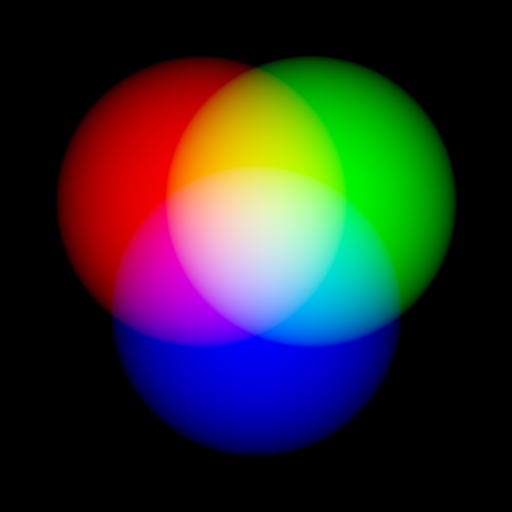
\includegraphics[width=0.4\linewidth]{images/rgb-space.png}
            \caption{ภาพสีเกิดจากการผสมกันระหว่างสี แดง เขียว และน้ำเงิน\footnote{\tiny{ภาพจาก \url{https://commons.wikimedia.org/wiki/File:Additive_RGB_Circles-48bpp.png}  สืบค้นเมื่อวันที่ 25 กันยายน 2561}}}
            \label{image:rgb-space}
        \end{figure}
    \end{frame}
    \begin{frame}
        \frametitle{ภาพสี (ต่อ)}
        \begin{align*}
             \boldsymbol{u},\ \boldsymbol{z} : \Omega  \rightarrow V
        \end{align*}
        \begin{align*}
            \Big \downarrow
        \end{align*}
        \begin{align*}
             \boldsymbol{u} = \begin{bmatrix} \textcolor{red}{u_1} \\ \textcolor{OliveGreen}{u_2} \\ \textcolor{blue}{u_3}   \end{bmatrix}, \ \boldsymbol{z} =\begin{bmatrix} \textcolor{red}{z_1} \\ \textcolor{OliveGreen}{z_2} \\ \textcolor{blue}{z_3} \end{bmatrix} : \Omega  \rightarrow V^3
        \end{align*} 
    \end{frame}
    \begin{frame}
        \frametitle{ตัวแบบการต่อเติมภาพสีที่ใช้การแปรผันรวม}
        \begin{align*}
        \min_{u} \{ \mathcal{J}(u) = \frac{1}{2} \int_{\Omega}\lambda (u-z)^2 d\Omega +  \int_{\Omega}  |\nabla u|  d\Omega \}
        \end{align*}
        \begin{align*}
        \Big \downarrow
        \end{align*}
        \begin{align*}
        \min_{u} \{ \mathcal{J}(u) = \underset{l=1}{\overset{3}{\sum}} 
        ( \frac{1}{2} \int_{\Omega}\lambda (u_l-z_l)^2 d\Omega +  \int_{\Omega}  |\nabla u_l|  d\Omega ) \}
        \end{align*}
    \end{frame}
    \begin{frame}
    \frametitle{วิธีการสปริทเบรกแมนสำหรับภาพสี}
        \begin{align*}
        \min_{u,\boldsymbol{w}} \{ \mathcal{J}(u,\boldsymbol{w}) = \dfrac{1}{2} \int_{\Omega} \lambda(u-z)^2 d\Omega +  \int_{\Omega}  |\nabla \boldsymbol{w}|  d\Omega + \frac{\theta}{2} \int_{\Omega} (\boldsymbol{w} - \nabla u + \boldsymbol{b}) d\Omega \}
        \end{align*}
        \begin{align*}
        \Big \downarrow
        \end{align*}
        \begin{align*}
        \min_{\boldsymbol{u},\boldsymbol{w_1},\boldsymbol{w_2},\boldsymbol{w_3}} \{ \mathcal{J}(\boldsymbol{u},\boldsymbol{w_1},\boldsymbol{w_2},\boldsymbol{w_3}) &= \underset{l=1}{\overset{3}{\sum}} (  \dfrac{1}{2} \int_{\Omega} \lambda(u_l-z_l)^2 d\Omega +  \int_{\Omega}  |\nabla \boldsymbol{w_l}|  d\Omega \\ &+ \frac{\theta}{2} \int_{\Omega} (\boldsymbol{w_l} - \nabla u_l+ \boldsymbol{b_l}) d\Omega ) \}
        \end{align*}
    \end{frame}
    \begin{frame}
        \frametitle{Peak Signal Noise Ratio (PSNR)}
        \begin{align*}
        \text{PSNR}  = 10 \cdot log_{10} ( \frac{1}{\sqrt{\text{MSE}}} )  \hspace{1cm}
        \end{align*}
        \begin{itemize}
            \item[$\bullet$] MSE คือค่าคลาดเคลื่อนกำลังสองเฉลี่ยของภาพ โดยที่ MSE = $\frac{1}{nx \times ny} \sum (u - \tilde{u})^2 $
            \item[$\bullet$] $u$ แทนภาพต้นฉบับ
            \item[$\bullet$] $\tilde{u}$  แทนภาพที่ได้จากการซ่อมแซมโดยวิธีเชิงตัวเลข
            \item[$\bullet$] PSNR มีหน่วยเป็น dB
        \end{itemize}
    \end{frame}
    \begin{frame}
        \frametitle{Structural Similarity (SSIM)}
        \begin{align*}
        \text{SSIM}(u,\tilde{u}) = \frac{(2\mu_u\mu_{\tilde{u}} + 0.0001)(2\sigma_{u\tilde{u}} + 0.0009)}{(\mu_u^2+\mu_{\tilde{u}}^2+0.0001)(\sigma_u^2+\sigma_{\tilde{u}}^2+0.0009)}
        \end{align*}
        \begin{itemize}
            \item[$\bullet$] $u$ แทนภาพต้นฉบับ
            \item[$\bullet$] $\tilde{u}$  แทนภาพต้นฉบับ และภาพที่ได้จากการซ่อมแซมโดยวิธีเชิงตัวเลข
            \item[$\bullet$] $\mu_u$ คือค่าเฉลี่ยของ $u$
            \item[$\bullet$] $\mu_{\tilde{u}}$ คือค่าเฉลี่ยของ $\tilde{u}$
            \item[$\bullet$]  $\sigma_u$ คือความแปรปรวนของ $u$ 
            \item[$\bullet$] $\sigma_{\tilde{u}}$ คือความแปรปรวนของ $\tilde{u}$
        \end{itemize}
    \end{frame}
    \begin{frame}
        \frametitle{ภาพสังเคราะห์}
        \begin{figure}[H]
            \centering
            \begin{subfigure}{0.15\linewidth}
                \centering
                
\includegraphics[width=0.9\linewidth]{images/image_inpaint_synthetic/case01-original.png}
            \end{subfigure}
            \begin{subfigure}{0.15\linewidth}
                \centering
                
\includegraphics[width=0.9\linewidth]{images/image_inpaint_synthetic/case02-original.png}
            \end{subfigure}
            \begin{subfigure}{0.15\linewidth}
                \centering
                
\includegraphics[width=0.9\linewidth]{images/image_inpaint_synthetic/case03-original.png}	
            \end{subfigure}
            \begin{subfigure}{0.15\linewidth}
                \centering
                
\includegraphics[width=0.9\linewidth]{images/image_inpaint_synthetic/case04-original.png}
            \end{subfigure}
            \begin{subfigure}{0.15\linewidth}
                \centering
                
\includegraphics[width=0.9\linewidth]{images/image_inpaint_synthetic/case05-original.png}	
            \end{subfigure}
            \caption{ภาพต้นฉบับ}
        \end{figure}
        \begin{figure}[H]
            \centering
            \begin{subfigure}{0.15\linewidth}
                \centering
                
\includegraphics[width=0.9\linewidth]{images/image_inpaint_synthetic/case01-toinpaint.png}
            \end{subfigure}
            \begin{subfigure}{0.15\linewidth}
                \centering
                
\includegraphics[width=0.9\linewidth]{images/image_inpaint_synthetic/case02-toinpaint.png}
            \end{subfigure}
            \begin{subfigure}{0.15\linewidth}
                \centering
                
\includegraphics[width=0.9\linewidth]{images/image_inpaint_synthetic/case03-toinpaint.png}
            \end{subfigure}
            \begin{subfigure}{0.15\linewidth}
                \centering
                
\includegraphics[width=0.9\linewidth]{images/image_inpaint_synthetic/case04-toinpaint.png}
            \end{subfigure}
            \begin{subfigure}{0.15\linewidth}
                \centering
                
\includegraphics[width=0.9\linewidth]{images/image_inpaint_synthetic/case05-toinpaint.png}
            \end{subfigure}
            \caption{ภาพที่จะทำการซ่อมแซม}
        \end{figure}
        \begin{align*}
            \text{รอบการทำซ้ำ} \leq 10,000 \text{รอบ} \hspace{1cm}
            \frac{|| u_{new} - u_{old} ||}{|| u_{new} ||} \geq 10^{-4}
        \end{align*}
    \end{frame}
    \begin{frame}
        \frametitle{ผลการต่อเติมภาพ}
        \begin{figure}[H]
            \centering
            \begin{subfigure}{0.15\linewidth}
                \centering
                
\includegraphics[width=0.9\linewidth]{images/result_ex1/timemarch01.png}
            \end{subfigure}
            \begin{subfigure}{0.15\linewidth}
                \centering
                
\includegraphics[width=0.9\linewidth]{images/result_ex1/timemarch02.png}
            \end{subfigure}
            \begin{subfigure}{0.15\linewidth}
                \centering
                
\includegraphics[width=0.9\linewidth]{images/result_ex1/timemarch03.png}
            \end{subfigure}
            \begin{subfigure}{0.15\linewidth}
                \centering
                
\includegraphics[width=0.9\linewidth]{images/result_ex1/timemarch04.png}
            \end{subfigure}
            \begin{subfigure}{0.15\linewidth}
                \centering
                
\includegraphics[width=0.9\linewidth]{images/result_ex1/timemarch05.png}
            \end{subfigure}
            \caption{ผลการซ่อมแซมจากวิธีการเดินเวลา}
        \end{figure}
        \begin{figure}[H]
            \centering
            \begin{subfigure}{0.15\linewidth}
                \centering
                
\includegraphics[width=0.9\linewidth]{images/result_ex1/fixpoint01.png}
            \end{subfigure}
            \begin{subfigure}{0.15\linewidth}
                \centering
                
\includegraphics[width=0.9\linewidth]{images/result_ex1/fixpoint02.png}
            \end{subfigure}
            \begin{subfigure}{0.15\linewidth}
                \centering
                
\includegraphics[width=0.9\linewidth]{images/result_ex1/fixpoint03.png}
            \end{subfigure}
            \begin{subfigure}{0.15\linewidth}
                \centering
                
\includegraphics[width=0.9\linewidth]{images/result_ex1/fixpoint04.png}
            \end{subfigure}
            \begin{subfigure}{0.15\linewidth}
                \centering
                
\includegraphics[width=0.9\linewidth]{images/result_ex1/fixpoint05.png}
            \end{subfigure}
            \caption{ผลการซ่อมแซมจากวิธีการทำซ้ำแบบจุดตรึง}
        \end{figure}
        \begin{figure}[H]
            \centering
            \begin{subfigure}{0.15\linewidth}
                \centering
                
\includegraphics[width=0.9\linewidth]{images/result_ex1/splitbergman01.png}
            \end{subfigure}
            \begin{subfigure}{0.15\linewidth}
                \centering
                
\includegraphics[width=0.9\linewidth]{images/result_ex1/splitbergman02.png}
            \end{subfigure}
            \begin{subfigure}{0.15\linewidth}
                \centering
                
\includegraphics[width=0.9\linewidth]{images/result_ex1/splitbergman03.png}
            \end{subfigure}
            \begin{subfigure}{0.15\linewidth}
                \centering
                
\includegraphics[width=0.9\linewidth]{images/result_ex1/splitbergman04.png}
            \end{subfigure}
            \begin{subfigure}{0.15\linewidth}
                \centering
                
\includegraphics[width=0.9\linewidth]{images/result_ex1/splitbergman05.png}
            \end{subfigure}
            \caption{ผลการซ่อมแซมจากวิธีการสปริทเบรกแมน}
        \end{figure}
    \end{frame}
    \begin{frame}
        \frametitle{ประสิทธิภาพของวิธีการเชิงตัวเลขทั้ง 3 วิธี}
        \begin{table}[H]
        \centering
        \captionsetup{justification=centering}
            \begin{tabular}[ht]{|l|c|c|c|c|}
                \hline
                วิธีการ  & เวลาประมวล  (วินาที) & PSNR (dB) & SSIM \\
                \hline
                การเดินเวลา & 120.68 & 16.72 & 0.9960 \\
                การทำซ้ำจุดตรึง & 74.81 & 38.67 & 0.9999 \\
                การสปริทเบรกแมน & 14.06 & 39.42 & 0.9999  \\
                \hline
            \end{tabular}
        \caption{แสดงการซ่อมแซมเฉลี่ยของวิธีการเชิงตัวเลข \\ โดยที่ $\lambda = 250, \beta = 10^{-5}, \tau = 10^{-5}, \theta = 5 $}
        \end{table}	
    \end{frame}
    \begin{frame}
        \frametitle{คำตอบเริ่มต้น (intial solution)}
        \begin{figure}[H]
            \centering
            \begin{subfigure}{0.8\linewidth}
                \centering
                
\includegraphics[width=1\linewidth]{images/image_inpaint_synthetic/image_inital_solution.png}
            \end{subfigure}
            \caption{สร้างคำตอบเริ่มต้นโดยใช้พีระมิดรูปภาพ}
        \end{figure}
    \end{frame}
    \begin{frame}
        \frametitle{พีระมิดรูปภาพ}
        \begin{figure}[H]
            \centering
            \begin{subfigure}{0.6\linewidth}
                \centering
                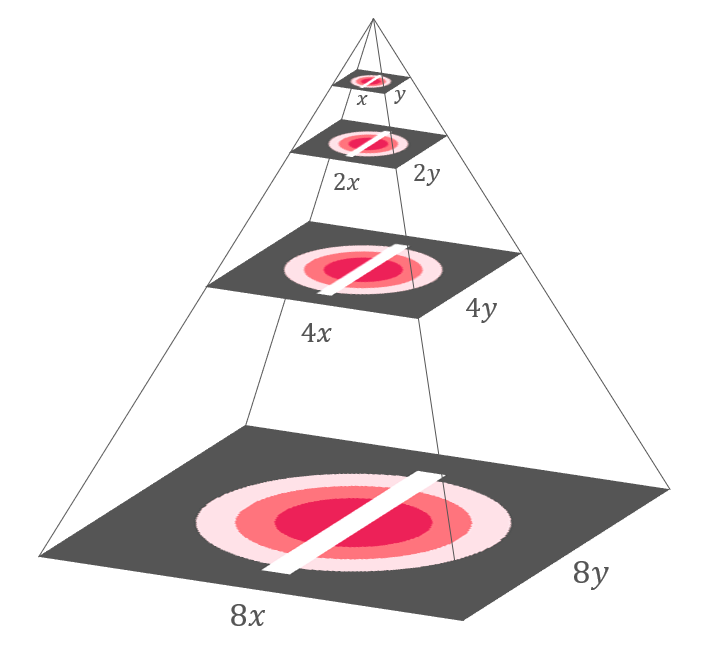
\includegraphics[width=0.8\linewidth]{images/image_inpaint_synthetic/image_pyramid.png}
            \end{subfigure}
            \caption{วิธีการพีระมิดรูปภาพ}
        \end{figure}
        \let\thefootnote\relax\footnotetext{\tiny{	E.H. Andelson and C.H. Anderson and J.R. Bergen and P.J. Burt and J.M. Ogden. "Pyramid methods in image processing". 1984}}
    \end{frame}
    \begin{frame}
        \frametitle{ผลการซ่อมแซมเมื่อใช้พีระมิดรูปภาพ}
        \begin{table}[H]
            \centering
            \begin{tabular}[ht]{|l|c|c|c|c|}
                \hline
                รูปแบบการทำซ้ำ  & เวลาประมวล  (วินาที) & PSNR (dB) & SSIM \\
                \hline
                ไม่ใช้พีระมิดรูปภาพ & 17.38 & 39.42 & 0.9999 \\
                10/1/1/10000 & 13.52 & 39.38 & 0.9999 \\
                10/3/3/10000 & 11.86 & 39.54 & 0.9999 \\
                10/10/10/10000 & 9.26 & 40.17 & 0.9999\\
                100/1/1/10000 & 10.28 & 39.04 & 0.9999\\
                100/3/3/10000 & 10.28 & 39.80 & 0.9999\\
                100/10/10/10000 & 9.27 & 40.12 & 0.9999 \\
                \hline
            \end{tabular}
            \caption{ผลการซ่อมแซมภาพโดยวิธีการเชิงตัวเลขที่นำเสนอในรูปของค่าเฉลี่ย}
            \label{result:table-multiresolution1-summary}
        \end{table}	
    \end{frame}
    \begin{frame}
        \frametitle{การทำซ้ำความละเอียดคมชัดสุด}
        \begin{figure}[H]
            \centering
            \begin{subfigure}{0.4\linewidth}
                \centering
                
\includegraphics[width=0.6\linewidth]{images/just10enough/only5time.png}
                \caption{5 ครั้ง}
            \end{subfigure}
            \begin{subfigure}{0.4\linewidth}
                \centering
                
\includegraphics[width=0.6\linewidth]{images/just10enough/only10time.png}
                \caption{10 ครั้ง}
            \end{subfigure}
            \begin{subfigure}{0.4\linewidth}
                \centering
                
\includegraphics[width=0.6\linewidth]{images/just10enough/only50time.png}			
                \caption{50 ครั้ง}
            \end{subfigure}
            \begin{subfigure}{0.4\linewidth}
                \centering
                
\includegraphics[width=0.6\linewidth]{images/just10enough/only100time.png}			
                \caption{100 ครั้ง}
            \end{subfigure}
            \caption{{\footnotesize พีระมิดที่ลำดับการทำซ้ำเป็น 10/10/10 และที่ระดับความคมชัดละเอียดสุดใช้จำนวนการทำซ้ำที่ต่างกัน}}
        \end{figure}
    \end{frame}
    \begin{frame}
        \frametitle{ผลการซ่อมแซมภาพในระดับความคมชัดละเอียดสุด 10 ครั้ง}
        \begin{table}[H]
            \centering
            \begin{tabular}[ht]{|l|c|c|c|c|}
                \hline
                รูปแบบการทำซ้ำ  & เวลาประมวล  (วินาที) & PSNR (dB) & SSIM \\
                \hline
                ไม่ใช้พีระมิดรูปภาพ & 0.37 & 17.26 & 0.9963  \\
                10/1/1/10 & 0.40 & 28.54 & 0.9993 \\
                10/3/3/10 & 0.33 & 29.83  & 0.9994 \\
                10/10/10/10 & 0.38 & 32.56 & 0.9995 \\
                100/1/1/10 & 0.34 & 31.50 & 0.9999 \\
                100/3/3/10 & 0.36 & 31.99 & 0.9999 \\
                100/10/10/10 & 0.38 & 33.39 & 0.9998 \\
                \hline
            \end{tabular}
            \caption{{\small ผลการซ่อมแซมภาพเฉลี่ยเมื่อใช้การทำซ้ำในระดับความคมชัดละเอียดสุด 10 ครั้ง}}
        \end{table}	
    \end{frame}
    \begin{frame}
        \frametitle{การซ่อมแซมภาพจิตรกรรมไทยโบราณ}
        \begin{figure}[H]
            \centering
            \begin{subfigure}{0.15\linewidth}
                \centering
                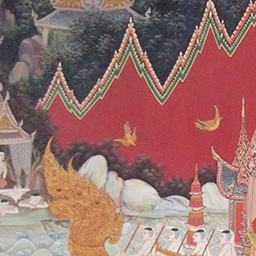
\includegraphics[width=0.9\linewidth]{images/thaiart/case01-original.png}
            \end{subfigure}
            \begin{subfigure}{0.15\linewidth}
                \centering
                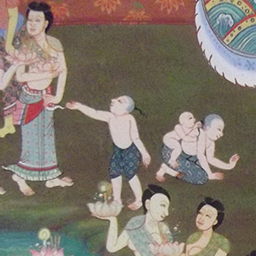
\includegraphics[width=0.9\linewidth]{images/thaiart/case02-original.png}
            \end{subfigure}
            \begin{subfigure}{0.15\linewidth}
                \centering
                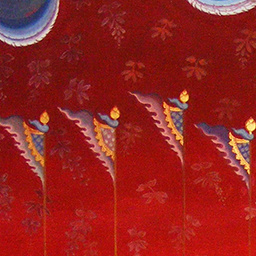
\includegraphics[width=0.9\linewidth]{images/thaiart/case03-original.png}
            \end{subfigure}		
            \begin{subfigure}{0.15\linewidth}
                \centering
                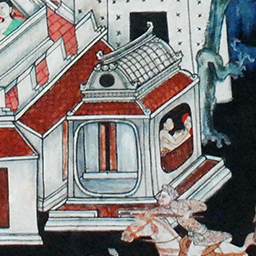
\includegraphics[width=0.9\linewidth]{images/thaiart/case04-original.png}
            \end{subfigure}
            \begin{subfigure}{0.15\linewidth}
                \centering
                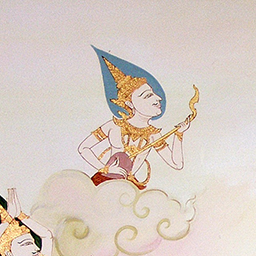
\includegraphics[width=0.9\linewidth]{images/thaiart/case05-original.png}
            \end{subfigure}
            \caption{ภาพต้นฉบับสำหรับใช้ในการทดสอบ}
        \end{figure}
        \begin{figure}[H]
            \centering
            \begin{subfigure}{0.15\linewidth}
                \centering
                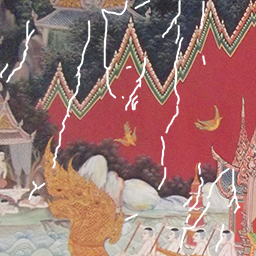
\includegraphics[width=0.9\linewidth]{images/thaiart/case01-toinpaint.png}
            \end{subfigure}
            \begin{subfigure}{0.15\linewidth}
                \centering
                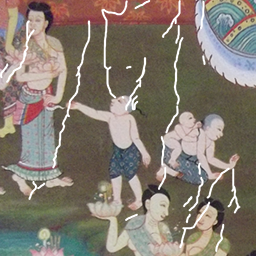
\includegraphics[width=0.9\linewidth]{images/thaiart/case02-toinpaint.png}
            \end{subfigure}
            \begin{subfigure}{0.15\linewidth}
                \centering
                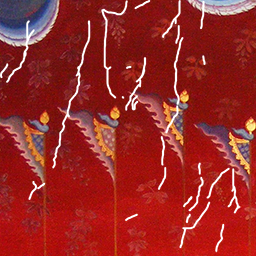
\includegraphics[width=0.9\linewidth]{images/thaiart/case03-toinpaint.png}			
            \end{subfigure}
            \begin{subfigure}{0.15\linewidth}
                \centering
                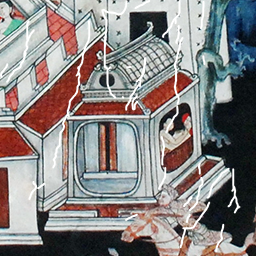
\includegraphics[width=0.9\linewidth]{images/thaiart/case04-toinpaint.png}			
            \end{subfigure}
            \begin{subfigure}{0.15\linewidth}
                \centering
                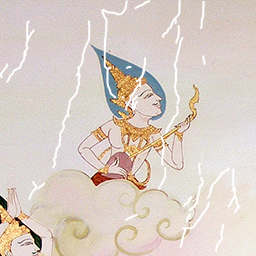
\includegraphics[width=0.9\linewidth]{images/thaiart/case05-toinpaint.png}			
            \end{subfigure}
            \caption{ภาพที่ทำให้เสียหาย}
        \end{figure}
    \end{frame}
    \begin{frame}
        \frametitle{ผลการซ่อมแซมภาพศิลปะไทย}
        \begin{figure}[H]
            \centering
            \begin{subfigure}{0.15\linewidth}
                \centering
                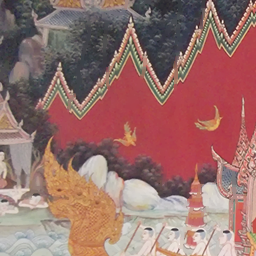
\includegraphics[width=0.9\linewidth]{images/result_ex4/splitbergman_case01.png}
            \end{subfigure}
            \begin{subfigure}{0.15\linewidth}
                \centering
                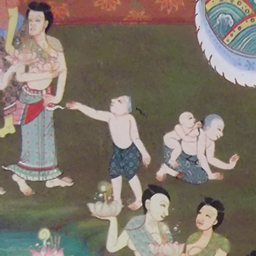
\includegraphics[width=0.9\linewidth]{images/result_ex4/splitbergman_case02.png}
            \end{subfigure}
            \begin{subfigure}{0.15\linewidth}
                \centering
                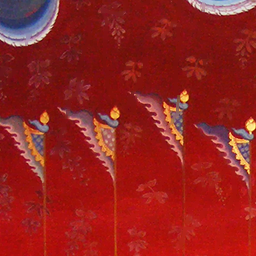
\includegraphics[width=0.9\linewidth]{images/result_ex4/splitbergman_case03.png}			
            \end{subfigure}
            \begin{subfigure}{0.15\linewidth}
                \centering
                \includegraphics[width=0.9\linewidth]{images/result_ex4/splitbergman_case04.png}			
            \end{subfigure}
            \begin{subfigure}{0.15\linewidth}
                \centering
                \includegraphics[width=0.9\linewidth]{images/result_ex4/splitbergman_case05.png}			
            \end{subfigure}
            \caption{ผลการซ่อมแซมโดยวิธีการสปริทเบรกแมน}
        \end{figure}
        \begin{figure}[H]
            \centering
            \begin{subfigure}{0.15\linewidth}
                \centering
                \includegraphics[width=0.9\linewidth]{images/result_ex4/multisplitbergman_case01.png}
            \end{subfigure}
            \begin{subfigure}{0.15\linewidth}
                \centering
                \includegraphics[width=0.9\linewidth]{images/result_ex4/multisplitbergman_case02.png}
            \end{subfigure}
            \begin{subfigure}{0.15\linewidth}
                \centering
                \includegraphics[width=0.9\linewidth]{images/result_ex4/multisplitbergman_case03.png}			
            \end{subfigure}
            \begin{subfigure}{0.15\linewidth}
                \centering
                \includegraphics[width=0.9\linewidth]{images/result_ex4/multisplitbergman_case04.png}			
            \end{subfigure}
            \begin{subfigure}{0.15\linewidth}
                \centering
                \includegraphics[width=0.9\linewidth]{images/result_ex4/multisplitbergman_case05.png}			
            \end{subfigure}
            \caption{ผลการซ่อมแซมโดยวิธีการที่พัฒนาขึ้น}
        \end{figure}
    \end{frame}
    \begin{frame}
        \frametitle{เปรียบเทียบระหว่าง 2 วิธี}
        \begin{figure}[H]
            \centering
            \begin{subfigure}{0.4\linewidth}
                \centering
                \includegraphics[width=0.6\linewidth]{images/result_ex4_scaleup/original.png}
                \caption{ภาพต้นฉบับ}
            \end{subfigure}
            \begin{subfigure}{0.4\linewidth}
                \centering
                \includegraphics[width=0.6\linewidth]{images/result_ex4_scaleup/toinpaint.png}
                \caption{ภาพที่เสียหาย}
            \end{subfigure}
            \begin{subfigure}{0.4\linewidth}
                \centering
                \includegraphics[width=0.6\linewidth]{images/result_ex4_scaleup/splitbregman.png}			
                \caption{วิธีสปริทเบรกแมน}
            \end{subfigure}
            \begin{subfigure}{0.4\linewidth}
                \centering
                \includegraphics[width=0.6\linewidth]{images/result_ex4_scaleup/multisplitbregman.png}	
                \caption{วิธีที่พัฒนาขึ้น}
            \end{subfigure}
            \caption{เปรียบเทียบจากภาพที่ถูกขยายขึ้น 4 เท่า}
        \end{figure}
    \end{frame}
    \begin{frame}
        \frametitle{ผลการซ่อมแซมภาพศิลปะไทย}
        % เร็วกว่าประมาณ 7 เท่า
        \begin{table}[H]
            \centering
            \begin{tabular}[ht]{|l|c|c|c|c|}
                \hline
                วิธีการ  & เวลาประมวล  (วินาที) & PSNR (dB) & SSIM \\
                \hline
                สปริทเบรกแมน & 2.72 & 34.89 & 1.0000 \\ 
                วิธีการที่พัฒนาขึ้น & 0.39 & 35.30 & 1.0000 \\
                \hline
            \end{tabular}
            \caption{แสดงผลการซ่อมแซมภาพศิลปะไทยในรูปค่าเฉลี่ย}
            \label{result:table-thaiart-summary}
        \end{table}	
    \end{frame}
    \begin{frame}
        \frametitle{การลบบทบรรยายบนอนิเมะ}
        \begin{figure}[H]
            \centering
            \includegraphics[width=0.8\linewidth]{images/inori-preview.png}
            \caption{ Festival Asia Special Video - feat. Inori Aizawa }
        \end{figure}
    \end{frame}
    \begin{frame}
        \frametitle{Lorem Ipsum}
            \begin{figure}[H]
            \centering
            \includegraphics[width=0.85\linewidth]{images/lorem4lang.png}
            \caption{Lorem Ipsum ทั้ง 4 ภาษา \footnote{ \tiny{ส่วนหนึ่งของ Lorem ipsum  ในภาษาต่างๆ จาก https://en.wikipedia.org/wiki/Lorem\_ipsum,  https://ja.wikipedia.org/wiki/Lorem\_ipsum และ  https://th.wikipedia.org/wiki/ลอเร็มอิปซัม สืบค้นเมื่อ 25 พฤศจิกายน 2561} } }
        \end{figure}
    \end{frame}
    \begin{frame}
        \frametitle{การแบ่งไฟล์วิดีโอ}
            \begin{figure}[H]
            \centering
            \includegraphics[width=0.8\linewidth]{images/inori-subbed-preview.png}
            \caption{แบ่งวิดีโอออกเป็น 5 ส่วน}
        \end{figure}
    \end{frame}
    \begin{frame}
    \frametitle{วิดีโอกับภาพ}
        \begin{figure}[H]
            \centering
            \includegraphics[width=0.6\linewidth]{images/anime-frame.png}
            \caption{วิดีโอคือลำดับของภาพ}
        \end{figure}
    \end{frame}
    \begin{frame}
        \frametitle{การหาบทบรรยาย}
        \begin{figure}[H]
            \centering
            \includegraphics[width=0.8\linewidth]{images/subtitle-remove/thisisanimesubtitle.png}
            \caption{บทบรรยายอนิเมะมักมีขอบเป็นสีดำ}
        \end{figure}
    \end{frame}
    \begin{frame}
        \frametitle{การหาบทบรรยาย (ต่อ)}
        \begin{figure}[H]
            \begin{subfigure}{0.4\linewidth}
                \centering
                \includegraphics[width=0.8\linewidth]{images/subtitle_detection/detection-original.png}
                \caption{ภาพเฟรมอนิเมะบริเวณที่มีบทบรรยาย}
            \end{subfigure}
            \begin{subfigure}{0.4\linewidth}
                \centering
                \includegraphics[width=0.8\linewidth]{images/subtitle_detection/detection-threshold.png}
                \caption{ให้สีดำในภาพเป็นสีขาว สีอื่นเป็นสีดำ }
            \end{subfigure}
            \begin{subfigure}{0.4\linewidth}
                \centering
                \includegraphics[width=0.8\linewidth]{images/subtitle_detection/detection-inverse.png}
                \caption{สลับสีขาวเป็นสีดำ สีดำเป็นสีขาว}
            \end{subfigure}
            \begin{subfigure}{0.4\linewidth}
                \centering
                \includegraphics[width=0.8\linewidth]{images/subtitle_detection/detection-blackfill.png}
                \caption{ภาพหลังทำการเปลี่ยนพื้นที่สีขาว}
            \end{subfigure}
            \begin{subfigure}{0.4\linewidth}
                \centering
                \includegraphics[width=0.8\linewidth]{images/subtitle_detection/detection-erode-opening.png}
                \caption{ลบสิ่งที่เล็กเกินไปหรือใหญ่เกินไป}
            \end{subfigure}
            \begin{subfigure}{0.4\linewidth}
                \centering
                \includegraphics[width=0.8\linewidth]{images/subtitle_detection/detection-stoke.png}
                \caption{ขยายโดเมนต่อเติมให้ครอบคลุม}
            \end{subfigure}
            \caption{ขั้นตอนวิธีการหาบทบรรยาย}
        \end{figure}
    \end{frame}
    \begin{frame}
        \frametitle{ผลลัพธ์การหาบทบรรยาย}
        \begin{table}[H]
            \centering
            \footnotesize
            \begin{tabular}[ht]{|l|c|c|c|c|}
                \hline
                ภาษา  & จำนวนพิกเซลในโดเมน & จำนวนพิกเซลที่ตรวจพบ & จำนวนพิกเซลที่ผิดพลาด & ร้อยละการผิดพลาด \\
                \hline
                ไทย & 23,222,220 & 24,083,125 & 2,141,201 & 9.22 \\
                อังกฤษ & 27,278,745 & 28,598,424 & 3,714,321 & 13.62 \\
                ญี่ปุ่น & 28,544,173 & 30,103,466 & 3,740,971 & 13.11 \\
                \hline
            \end{tabular}
            \caption{ความคลาดเคลื่อนเฉลี่ยของการหาโดเมนต่อเติม ในบทบรรยายภาษาต่างๆ}
        \end{table}	
    \end{frame}
    \begin{frame}
        \frametitle{ลำดับภาพกับคำตอบเริ่มต้น}
        \begin{figure}[H]
            \centering
            \includegraphics[width=0.8\linewidth]{images/skipborrow/frame_sequence.png}
            \caption{ลำดับภาพในวิดีโอบริเวณคำบรรยาย}
        \end{figure}
    \end{frame}
    \begin{frame}
        \frametitle{พิจารณาความคล้ายด้วย SSIM}
        \begin{figure}[H]
            \centering
            \begin{subfigure}{0.4\linewidth}
                \centering
                \includegraphics[width=0.95\linewidth]{images/skipborrow/prevframe.png}
                \caption{เฟรมก่อนหน้า}
                \label{image:ssim_location_prev}
            \end{subfigure}
            \begin{subfigure}{0.4\linewidth}
                \centering
                \includegraphics[width=0.95\linewidth]{images/skipborrow/currentframe.png}
                \caption{เฟรมปัจจุบัน}
                \label{image:ssim_location_curr}
            \end{subfigure}
            \bigskip
            \begin{subfigure}{0.4\linewidth}
                \centering
                \includegraphics[width=0.95\linewidth]{images/skipborrow/prevframeinverse.png}
                \caption{บริเวณคำนวณ SSIM ของเฟรมก่อนหน้า}
                \label{image:ssim_location_prev_inv}
            \end{subfigure}
            \begin{subfigure}{0.4\linewidth}
                \centering
                \includegraphics[width=0.95\linewidth]{images/skipborrow/currentframeinverse.png}
                \caption{บริเวณคำนวณ SSIM ของเฟรมปัจจุบัน}
                \label{image:ssim_location_curr_inv}
            \end{subfigure}
            \caption{บริเวณที่คำนวณ SSIM สำหรับการข้ามเฟรมและยืมเฟรม}
            \label{image:ssim_location}
        \end{figure}
    \end{frame}
    \begin{frame}
        \frametitle{การข้ามเฟรม}  
        \begin{figure}[H]
            \centering
            \includegraphics[width=0.6\linewidth]{images/skipborrow/flowchart-skip.png}
            \caption{ขั้นตอนวิธีการข้ามเฟรม}
        \end{figure}      
    \end{frame}
    \begin{frame}
        \frametitle{การยืมเฟรม}      
        \begin{figure}[H]
            \centering
            \includegraphics[width=0.6\linewidth]{images/skipborrow/flowchart-borrow.png}
            \caption{ขั้นตอนวิธีการยืมเฟรม}
        \end{figure}   
    \end{frame}
    \begin{frame}
        \frametitle{การข้ามเฟรมและยืมเฟรม}  
        \begin{figure}[H]
            \centering
            \includegraphics[width=0.6\linewidth]{images/skipborrow/flowchart-skipandborrow.png}
            \caption{ขั้นตอนวิธีการข้ามและยืมเฟรม}
        \end{figure}        
    \end{frame}
    \begin{frame}
    \end{frame}
    \begin{frame}
        \frametitle{ผลของวิธีข้ามเฟรมและยืมเฟรม}
        \begin{table}[H]
            \centering
            \begin{tabular}[ht]{|l|c|c|c|c|}
                \hline
                วิธีการ  & เวลาประมวล  (วินาที) & PSNR (dB) & SSIM \\
                \hline
                สปริทเบรกแมนและพีระมิดรูปภาพ & 141.29 & 31.39  &  0.9510\\
                ข้ามเฟรม & 89.29 & 29.07 & 0.9408 \\
                ยืมเฟรม & 132.78 & 32.20 & 0.9655\\
                ข้ามเฟรมและยืมเฟรม & 75.76 & 29.33 & 0.9454 \\
                \hline
            \end{tabular}
            \caption{การลบคำบรรยายเฉลี่ยด้วยวิธีต่างๆ}
        \end{table}	
    \end{frame}
    \begin{frame}
        \frametitle{ผลการลบคำบรรยาย}
        \begin{figure}[H]
            \centering
            \begin{subfigure}{0.4\linewidth}
                \centering
                \includegraphics[width=0.80\linewidth]{images/subtitle-remove/beforesubtitleremove.png}
                \caption{ก่อนลบคำบรรยาย}
                \label{image:ssim_location_prev}
            \end{subfigure}
            \begin{subfigure}{0.4\linewidth}
                \centering
                \includegraphics[width=0.80\linewidth]{images/subtitle-remove/aftersubtitleremove.png}
                \caption{หลังลบคำบรรยาย}
                \label{image:ssim_location_curr}
            \end{subfigure}
            %\caption{ก่อนลบคำบรรยายและหลังลบคำบรรยาย}
        \end{figure}
    \end{frame}
    \begin{frame}
        \frametitle{ผลการลบคำบรรยาย (ต่อ)}
        \begin{table}[H]
            \centering
            \captionsetup{justification=centering}
            \begin{tabular}[ht]{|l|c|c|c|c|}
                \hline
                วิธีการ  & เวลาประมวล  (วินาที) & PSNR (dB) & SSIM \\
                \hline
                สปริทเบรกแมน & 5073.08 & 32.88 & 0.9654 \\
                วิธีการที่พัฒนาขึ้น & 75.76 & 29.33 & 0.9454 \\
                \hline
            \end{tabular}
            \caption{ผลการลบบทบรรยายออกจากอนิเมะเฉลี่ย\\โดยวิธีการสปริทเบรกแมนและวิธีการที่พัฒนาขึ้น}
        \end{table}	
    \end{frame}
    \begin{frame}
        \frametitle{ลองซ่อมแซมภาพศิลปะ}
        \centering
        \begin{figure}[H]
            \centering
            \includegraphics[width=0.8\linewidth]{images/colab_sample.png}
            \caption{ลองใช้งานได้ที่ https://bit.ly/demothai}
        \end{figure}
    \end{frame}
    \begin{frame}
        \centering
        \Huge{ขอขอบคุณ}
    \end{frame}
\end{document}